\documentclass[12pt]{book} 

\usepackage{amsmath}
\usepackage{graphicx}
\usepackage{import}
\usepackage{amsfonts}
\usepackage{booktabs}

\setlength{\parindent}{0em}  % sets auto indent at new paragraph to none

\newcommand{\incfig}[1]{%
    \import{./figures/}{#1.pdf_tex}
}

\title{\coursetitle\linebreak\lecturename}
\author{\\Cain Susko\\ 
           \\ \\ \\
      Queen's University 
    \\School of Computing\\} 

%=-=-=-=-=-title-=-=-=-=-=%
\newcommand{\lecturename}{Cross Validating Linear Regression}
\newcommand{\coursetitle}{Linear Data Analysis}
%=-=-=-=-=-#####-=-=-=-=-=%

\begin{document}
\begin{titlepage}
        \maketitle
\end{titlepage}


\section*{a Validation of Linear Regression}
Validation is a way of assessing a linear regression. Cross validating linear regression means to validate a regression with a subset of it's
        data.

A common form of cross validation is $k$-fold cross validation, where  we cross reference with a subset of size $k$. This topic is covered in
        Monday, Week 5 Tutorial.

\subsection*{Recall}
Each observation is $\vec x_i$. A data matrix is a matrix of $m$ observations: 
\[
A = \begin{bmatrix} \vec x_1^\top\\\vec x_2^\top\\\vdots\\\vec x_m^\top\end{bmatrix} 
.\] 


\begin{align*}
        &\text{Linear Regression:} &A\vec u \approx \vec c\\
        &\text{Standardize Data:} &A\to X \wedge \vec c \to \vec y\\
        &\text{Standard Problem:} &X\vec w \approx \vec y
.\end{align*}

\paragraph{}
Validation is to confirm that output of a model is acceptable.
Linear Regression is done over the independent data in $A$ and the dependent data  $\vec y$.
The usual technique for Validation is the Root Mean Squares method. 
Given the proposed solution $\vec w$ is:
 \[
RMS\left( X,\vec y; \vec w \right) = \sqrt{\frac{[X\vec w - \vec y]^\top [X\vec w - \vec y]}{m}}  
.\] 
This measures the \textit{fit} of the model $\vec w$ to \textbf{all} data.
\pagebreak


\section*{b Training Sets and Testing Sets}
\textbf{Training} is defined as: using data to find $\vec w$.\\
\textbf{Testing} is to evaluate the model using  $\vec w$.

Previously, we used all data  $X,\vec y$ to find  $\vec w$ and to evaluate the regression.
Instead, we can leave one or $n$ observations of  $\vec x \in X$ and  $y\in\vec y$ out of our 
        training. Then, we can test using the left out observation.

Thus, we should `Hold Back' $\vec x_i, y_i$ and train on the remaining  $X\left( \vec x_{i+1}:end\right)$, then 
        test on $\vec x_i, y_i$. 
We can then repeat this for all observations where we test the data on the respective data left out.

This procedure detects `singleton' statistical outliers.

\section*{c $k$-fold Cross Validation of Linear Regression}
we shall explore what's called $k$-fold validation.

Consider: the partition of data:
\[
X = \begin{bmatrix} X_1\\X_2 \end{bmatrix} \vec y = \begin{bmatrix} \vec y_1\\ \vec y_2 \end{bmatrix}  
.\] 

Where we train two models:
\[
X_1\vec w_1\approx \vec y_1\;\;\;X_2\vec w_2 \approx \vec y_2
.\] 

To cross validate these models, we will use the data from each to test the other using RMS.
\[
RMS(X_2,\vec y_2;\vec w_1)\;\;\;RMS(X_1,\vec y_1;\vec w_2)
.\] 
these partitions 1 and 2 are called `folds', and thus this is 2 fold cross validation.
The rule is, for $i$ in range  $k$: train  $\vec w_i$ on  $data_{i\to [i+(k-1)]\text{mod} k}$ and test $w_i$ on  $data_{i-1}$.
Typical values of $k$ are 5 or 10. 
\pagebreak


\section*{d Example of Five Fold Validation}
Given a dataset derived from a 2D line with 2 outliers. With this data $\vec a$ we will first augment it to $\vec a \to A$
We will then solve the approximation  $A\vec u \approx \vec c$ and set the result to be $\hat{u}$.
 \begin{figure}[h]
         \centering
         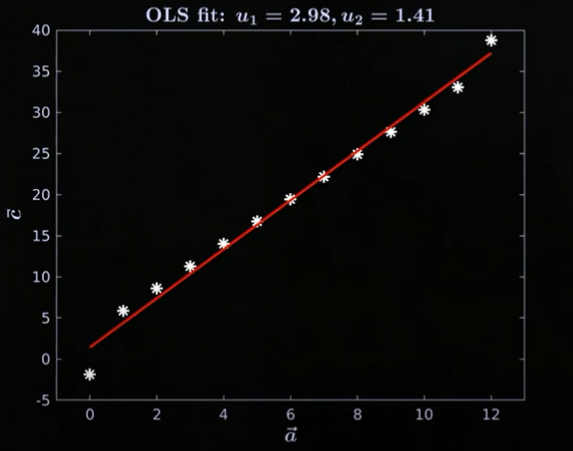
\includegraphics[scale=0.5]{./figures/RMS}
\end{figure}

Finally, we will compute the Root Mean Square Error $RMS(A,\vec c;\hat{u})$


Which results in a Root Mean Square Error of $1.3376$. 

But how valid is this RMSE?\@
If we do a five fold cross validation on the data where we train on $len(A)-5$ data and then test on $5$ data,
And then compare the mean of the RMSE of the training runs with that of the test runs.
\begin{figure}[h]
        \centering
        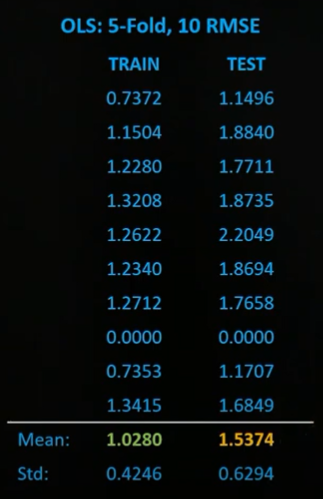
\includegraphics[scale=0.4]{./figures/RMSvalid}
\end{figure}

By the result we can see that the mean error of the training is less than the test error.
In fact, the error is about 50\% higher in testing than training.
This implies that the current model is not a good fit for the data.

\section*{Learning Summary}
Students should now be able to:
\begin{itemize}
        \item Validate linear regression with RMS Error
        \item Implement $k$-fold Cross Validation
        \item Assess the training errors and testing errors of a linear regression using cross validation
\end{itemize}

\end{document}

